\section{Abbildungen}\label{abbildungen} 

>>logo<< (vgl. Abb.~\ref{fig:logo}).% Referenz
  % Abb.
\begin{figure}[H]% hier: hbtp 
  \centering
  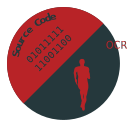
\includegraphics[width=0.7\textwidth]{images/logo}
  \caption{logo}%  Name
  \label{fig:logo}% Ref.
\end{figure}
  

>>logo-negativ<< (vgl. Abb.~\ref{fig:logo-negativ}).% Referenz
  % Abb.
\begin{figure}[H]% hier: hbtp 
  \centering
  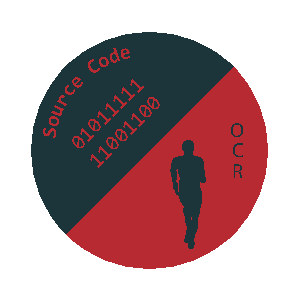
\includegraphics[width=0.7\textwidth]{images/logo-negativ}
  \caption{logo-negativ}%  Name
  \label{fig:logo-negativ}% Ref.
\end{figure}
  

>>Ordner-latex<< (vgl. Abb.~\ref{fig:Ordner-latex}).% Referenz
  % Abb.
\begin{figure}[H]% hier: hbtp 
  \centering
  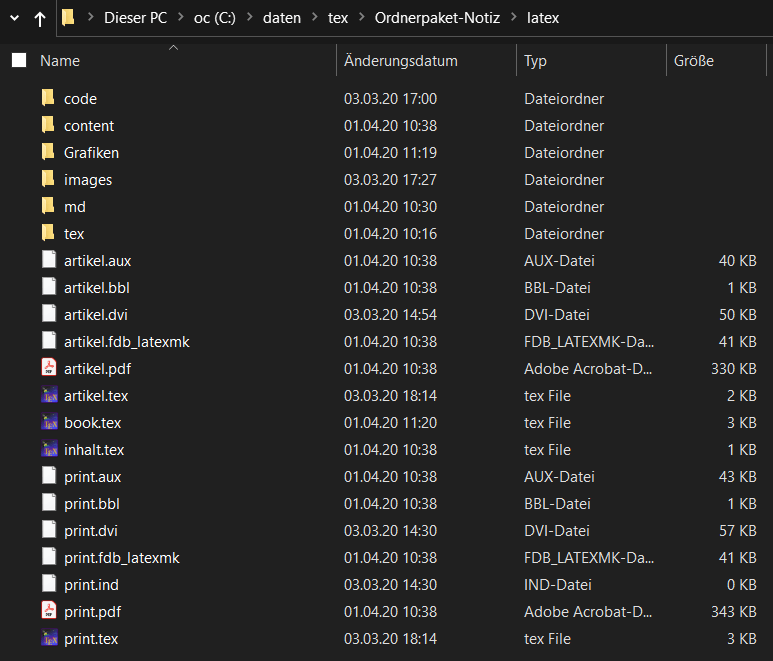
\includegraphics[width=0.7\textwidth]{images/Ordner-latex}
  \caption{Ordner-latex}%  Name
  \label{fig:Ordner-latex}% Ref.
\end{figure}
  

>>Ordner-struktur<< (vgl. Abb.~\ref{fig:Ordner-struktur}).% Referenz
  % Abb.
\begin{figure}[H]% hier: hbtp 
  \centering
  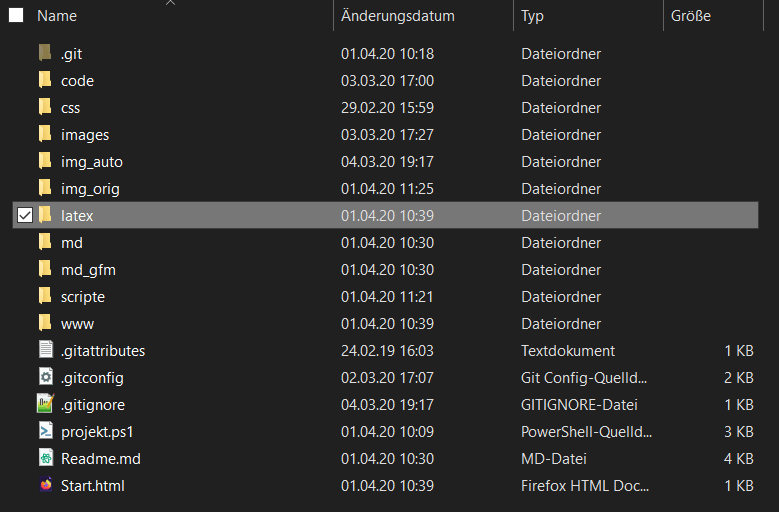
\includegraphics[width=0.7\textwidth]{images/Ordner-struktur}
  \caption{Ordner-struktur}%  Name
  \label{fig:Ordner-struktur}% Ref.
\end{figure}
  


